\section{Phase Quality and Path-Dependent Unwrapping}

\subsection{The Itoh Phase Unwrapping Algorithm}

\code{itk::ItohPhaseUnwrappingImageFilter} (defined in \code{itkItohPhaseUnwrappingImageFilter.h}) implements the simplest possible phase unwrapping algorithm, proposed by Itoh \cite{Itoh1982}.  In this algorithm, the image is traversed linearly, once per image dimension, unwrapping each pixel relative to the previous pixel.  In the case of the uncorrupted, wrapped phase ramp (Figure~\ref{fig:Simulated_Phase_Examples}, far left), the correct unwrapped image (Figure~\ref{fig:Simulated_Phase_Examples}, center left) is obtained with one traversal along the x direction (identical to input, not shown).  Additionally traversing along the y direction has no effect.  This is true regardless of which dimension is traversed first.

However, in the case of the noise-corrupted phase (Figure~\ref{fig:Itoh}), two notable observations should be made.  First, regardless of which direction is traversed first, the original phase image is not recovered.  Rather, the noisy region causes streaks to form `downstream' of the corrupted data.  Therefore, the Itoh algorithm is inadequate for unwrapping of this (and virtually all real world) data sets.  Second,  vertical followed by horizontal traversal does not produce the same image as the reverse.  This suggests that, whereas the unwrapping of some images (e.g., the uncorrupted phase ramp) is path-independent, the unwrapping of other images (e.g., the noisy-corrupted phase) is path-dependent.

\begin{figure}[h]
\center

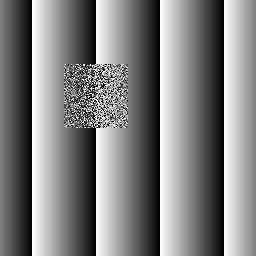
\includegraphics[width=0.24\textwidth]{images/2/00c_noise_wrapped.png}
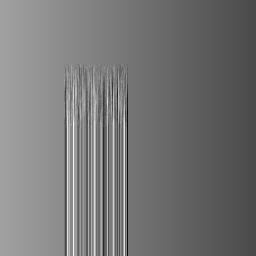
\includegraphics[width=0.24\textwidth]{images/3/01a_noise_xy.png}
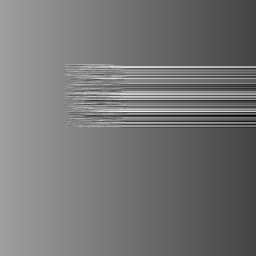
\includegraphics[width=0.24\textwidth]{images/3/01b_noise_yx.png}

\itkcaption[Itoh Phase Unwrapping Algorithm]{Noise-corrupted phase example ramps, unwrapped via the Itoh algorithm (\code{itk::ItohPhaseUnwrappingImageFilter}) in the horizontal then vertical directions (center) and in the vertical then horizontal directions (right).  The wrapped image (left) is reproduced for comparison.}
\label{fig:Itoh}
\end{figure}

\subsection{Phase Residues}

In order to predict when path-independent phase unwrapping is possible, it is necessary to introduce the concept of phase residues.  A residue charge is calculated for a 2x2 neighborhood of pixels and a given pair of dimensions, by summing the wrapped phase differences across a clockwise trajectory through the neighborhood and dividing the result by $2\pi$.\footnote{We here use the clockwise convention, as presented by Goldstein, et al \cite{Goldstein1988}.  However, as it is only the relative sign that is important for phase unwrapping, the clockwise/counter-clockwise convention makes no practical difference, so long as consistency is maintained.}  Effectively, this gives the number of positive discontinuities encountered less the number of negative discontinuities encountered (positive meaning that $2\pi$ would be added in order to remove it).

It has been proven that all phase residues have a value in the set $\left \{ -1, 0, 1\right \}$ \cite{Bone1991}.  Take the following minimal example (Figure~\ref{fig:Phase_Residues}):\footnote{For simplicity of calculation, the phase has been divided by $2\pi$ such that the range is from $(-0.5, 0.5]$ and the phase residues do not need to be rescaled.}

\begin{figure}[h]
\center
$\begin{matrix}

0.0 &  \rightarrow  & 0.3  &  \rightarrow & 0.3  &  \rightarrow  & 0.0 \\
\uparrow &  \odot  & \downarrow \uparrow &  & \downarrow \uparrow & \otimes & \downarrow \\
0.0 & \leftarrow   & -0.3 & \leftarrow  & -0.3 &  \leftarrow  & 0.0 \\

\end{matrix}$

\itkcaption[Phase_Residues]{Phase Residues.  Phase residues are calculated by summing the wrapped phase differences in a clockwise trajectory through a 2x2 neighborhood.  A positive residue ($\odot$) is noted in the leftmost neighborhood, a negative residue ($\otimes$) in the rightmost neighborhood, and no residue in the central neighborhood. }
\label{fig:Phase_Residues}
\end{figure}

The presence of one or more phase residues in a phase image denote path-dependent unwrapping.  In the above example, unwrapping along $(0,0) \rightarrow (1,0) \rightarrow (1,1)$ produces a value of $0.7$ for pixel $(1,1)$ ($-0.3 + 1.0 = 0.7)$, whereas unwrapping from $(0,0) \rightarrow (0,1) \rightarrow (1,1)$ produces a value of $-0.3$ because no phase wraps are encountered.\footnote{In accordance with ITK convention, the origin is taken to be the upper left corner of the image, and zero-indexing is used.}  Another useful result is that the wrapped line integral around a larger neighborhood yields the sum of the phase residues contained within that neighborhood.  In this example, the line integral is 0, which rightly reflects the presence of a single positive and a single negative residue.  Goldstein, et al \cite{Goldstein1988}, were the first to appreciate the significance of phase residues for path-dependency of phase unwrapping, by introducing the concept of residue `balancing' for 2D phase unwrapping.  They observed that, by defining branch cuts across which phase unwrapping was disallowed (either between residues of opposing sign or from a residue to the edge of the image), a subset of paths could be defined for which the wrapped line integral was zero (i.e., a subset of paths, none of which enclose an unbalanced residue).  Within this subset, any path taken will arrive at an identical unwrapped solution (to an arbitrary additive multiple of $2\pi$).

Appropriately balancing residues will ensure consistent, but not necessarily correct results \cite{Bone1991}.  All possible paths within a specific configuration yield the same result, to an additive multiple of $2\pi$.  However, results are not necessarily consistent between branch-cut configurations.  Figure~\ref{fig:Branch_Cuts} illustrates this point.  Two possible branch cut configurations are shown, each with one possible phase unwrapping path.  It is noteworthy that the values of pixels $(1,1)$ and $(2,1)$ differ between the two configurations.

\begin{figure}[h]
\center

\begin{tabular}{@{}c@{}}
  
  $\begin{matrix}

0.0 &  \rightarrow  & 0.3  &  \rightarrow & 0.3  &  \rightarrow  & 0.0 \\
 & \odot & \textrm{---} &  & \textrm{---} & \otimes & \downarrow \\
0.0 & \leftarrow   & -0.3 & \leftarrow  & -0.3 &  \leftarrow  & 0.0 \\

\end{matrix}$

\\
\small (a)

\end{tabular}

\vspace{\floatsep}

\begin{tabular}{@{}c@{}}


$\begin{matrix}

0.0 &  \rightarrow  & 0.3  &  & 0.3  &  \rightarrow  & 0.0 \\
\uparrow & \odot & \downarrow &  & \uparrow & \otimes & \downarrow \\
0.0 & |   & 0.7 & \rightarrow  & 0.7 &  |  & 0.0 \\

\end{matrix}$

\\
\small (b)

\end{tabular}


\itkcaption[Branch_Cuts]{Branch Cut Configurations.  The above example demonstrates two possible branch cut configurations.  Configuration (a) connects residues of opposing sign to one another.  Configuration (b) connects each residue to the image border.  For each configuration, one possible unwrapping path is demonstrated.  `---' and `$|$' represent vertical and horizontal branch cuts, respectively; arrows represent the path of phase unwrapping.}
\label{fig:Branch_Cuts}
\end{figure}

It should also be noted that the branch cutting theory so far discussed in this section is specific to two dimensional phase unwrapping.  An extension of the branch cutting concept to three dimensions has been proposed \cite{Huntley2001}, which requires phase residues to be calculated with respect to each pair of dimensions (xy, xz, yz).  To our knowledge, the branch cutting method has not been extended to higher dimensions.  We have included a discussion of residues for completeness, and because we believe that the concepts are essential to the understanding of path dependence.  However, as our interest in this submission is with phase unwrapping filters that may be implimented over images of arbitrary dimension, no branch cutting algorithms have been included.

Phase residues may be calculated using the \code{itk::PhaseResidueImageFilter} class (defined in \code{itkPhaseResidueImageFilter.h} (Figure~\ref{fig:Phase_Residues_Noise_Patch}).  The filter inherits from \code{itk::PhaseImageToImageFilter}, and uses the \code{Wrap()} method to calculate phase residues as described above.  Note that, due to the theoretical limitations described above, the filter only has a clear physical significance for 2D images.

\begin{figure}[h]
\center
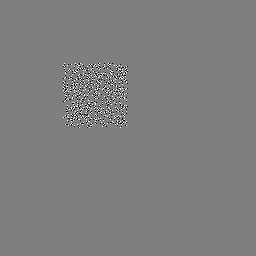
\includegraphics[width=0.24\textwidth]{images/3/02a_residue.png}

\itkcaption[Phase_Residues_Noise_Patch]{Phase residues are calculated for the noise-corrupted phase ramp example using the \code{itk::PhaseResidueImageFilter} class.}
\label{fig:Phase_Residues_Noise_Patch}
\end{figure}

\subsection{The Helmholtz Decomposition}

Given a vector field $v$, if there exists some $A$ such that $v = \nabla \times A$, then $A$ is called the `vector potential' of $v$.  Given that the divergence of the curl of any vector field is the zero vector, $v$ must therefore be entirely rotational (i.e., non-conservative):

\begin{equation}
\label{eqn:Div_Curl_Identity}
\nabla \cdot v = \nabla \cdot ( \nabla \times A ) = 0
\end{equation}

Likewise, if there exists some $\psi$ such that $v = \nabla \psi$, then $\psi$ is called the `scalar potential' of $v$.  Given that the curl of the gradient of any scalar field is zero, $v$ must therefore be entirely irrotational (i.e., conservative):

\begin{equation}
\label{eqn:Curl_Grad_Identity}
\nabla \times v = \nabla \times ( \nabla \psi ) = 0
\end{equation}

In the general case, $A$ and $\psi$ cannot be found (that is, the general case of a vector field need not be entirely rotational or irrotational).  However, the Helmholtz Decomposition states that a vector field can be decomposed into rotational and irrotational components as the sum of scalar and vector potentials:

\begin{equation}
\label{eqn:Helmholtz}
v = - \nabla \psi + \nabla \times A
\end{equation}

In the context of phase unwrapping, the Helmholtz decomposition has specific implications for path dependence.  In particular, the `path-dependent' contribution is contained entirely within the rotational component, and the `path-independent' contribution within the irrotational component.  The irrotational and rotational components of the noise-corrupted phase ramp are shown in the left and right panels of Figure~\ref{fig:Helmholtz_Decomposition}.  Note in the irrotational component that corruption of the original phase extends beyond the patch of noise itself, though there are no ambiguities.

\begin{figure}
\center
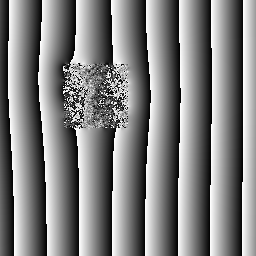
\includegraphics[width=0.24\textwidth]{images/3/02b_irrotational.png}
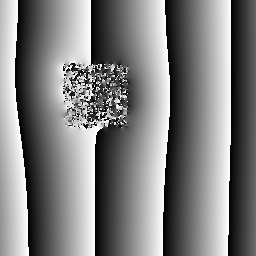
\includegraphics[width=0.24\textwidth]{images/3/02c_rotational.png}

\itkcaption[Helmholtz_Decomposition]{The \code{itk:HelmholtzDecompositionImageFilter} classe, applied to the noise-corrupted phase ramp example.  The left panel is the irrotational (curl-free) component, and the right panel is the rotational (divergence-free) component.}
\label{fig:Helmholtz_Decomposition}
\end{figure}

The Helmholtz Decomposition is provided in the \code{itk::HelmholtzDecompositionImageFilter} class (defined in \code{itkHelmholtzDecompositionImageFilter.h}), which inherits from \code{itk::PhaseImageToImagefilter}.  The irrotational and rotational components may be retrieved through the \code{GetRotational()} and \code{GetIrrotational()} methods, respectively.

The implementation of \code{itk::HelmholtzDecompositionImageFilter} takes advantage of the fact that the irrotational component is equivalent to the unweighted, least squares solution (\code{itk::DCTPhaseUnwrappingImageFilter}, discussed in a later section), re-wrapped into the range $(-\pi, \pi]$.  The rotational component may then be obtained by subtracting the irrotational component from the original wrapped phase, and re-wrapping the result.

\subsection{Phase Derivative Variance}

It addition to phase residues, it is also useful to consider continuous measures of phase quality, of which the phase derivative variance is the most commonly used.  Phase derivative variance $\sigma$ in a single dimension $d$ is the sum of squared differences of the local wrapped phase gradients ($\Delta \phi_{i}$) and the mean wrapped phase gradient ($\overline{ \Delta \phi }$, Equation~\ref{eqn:PhaseDerivativeVariance}). 

\begin{equation}
\label{eqn:PhaseDerivativeVariance}
\sigma_d = \sum_i{  \left( \Delta \phi_{i} - \overline{ \Delta \phi }     \right)^2  }
\end{equation}

The total phase derivative variance can then be found by dividing the sum of the root variance in each dimension by the square of the one-sided length of the neighborhood $k$ (Equation~\ref{eqn:PhaseDerivativeVarianceTotal}).  Phase derivative variance is a convenient measure of phase quality because it (a) is easily generalized to arbitrary dimension and (b) can be computed entirely from the phase data itself.

\begin{equation}
\label{eqn:PhaseDerivativeVarianceTotal}
\frac{ \sum_d { \sqrt{ \sigma_d } }  }{ k^2 }
\end{equation}

Phase derivative variance is an inverse measure of phase quality; i.e., a large phase derivative variance is indicative of low phase quality.  In order to be used as a quality metric, phase derivative variance is typically rescaled into the range $[0,1]$ and multiplied by $-1$, such that brighter pixels represent higher phase quality.  This is the default behavior of \code{itk::PhaseDerivativeVarianceImageFilter}.  The un-normalized phase derivative variance can be obtained by setting \code{SetNormalize(false)}.  The rescaled phase derivative variance image for the noise-corrupted phase ramp is shown in Figure~\ref{fig:Phase_Derivative_Variance}.

Note that the patch of noise can be clearly identified in the original wrapped image, the phase residue image, the phase derivative variance image, and the rotational component of the Helmholtz decomposition.

\begin{figure}[h]
\center
\fbox{ 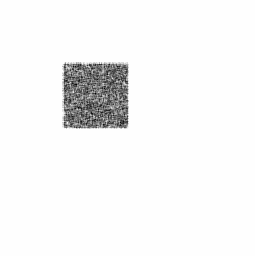
\includegraphics[width=0.24\textwidth]{images/3/02d_quality.png} }

\itkcaption[Phase_Derivative_Variance]{Phase Derivative Variance.  Rescaled phase derivative variance for the noise-corrupted phase ramp, computed with \code{itk::PhaseDerivativeVarianceImageFilter}.  The patch of noise can be clearly identified as a region of low image quality.  Note that a thin black border has been added in order to allow visualization of the edge of the image.}
\label{fig:Phase_Derivative_Variance}
\end{figure}
